\documentclass[dvipdfmx,20pt,notheorems,t]{beamer}
%\usepackage{bxdpx-beamer}
%\usepackage{pxjahyper}
\usepackage{minijs}
\renewcommand{\kanjifamilydefault}{\gtdefault}
\usetheme{boxes}
\usefonttheme{professionalfonts}
\setbeamertemplate{frametitle}[default][left]
\setbeamercovered{transparent}
\setbeamertemplate{footline}[page number]
\setbeamerfont{footline}{size=\normalsize,series=\bfseries}
\setbeamercolor{footline}{fg=black,bg=black}

\usepackage{amsmath,amssymb}
\usepackage{amsthm}
\theoremstyle{definition}


\title[ryaku]{(nil)}
\author[aa]{\textbf{@n\_IMRC}}
\institute[bb]{並木中等教育学校}
\date{\today}
\begin{document}
\begin{frame}[plain]\frametitle{}
\titlepage
\end{frame}

\begin{frame}\frametitle{自己紹介}
%\begin{alertblock}{monmon}
\begin{itemize}
\item 杉崎 行優
\item 並木中等教育学校 5年次
\item 筑波大学のスパコンCOMA利用者
\item Makefileガチ勢
\item Twitter: @n\_IMRC
\item Yo: IMRC
\item Github: Terminus-IMRC
\end{itemize}
%\end{alertblock}
\end{frame}

\begin{frame}\frametitle{今日話す内容}
\begin{itemize}
\item 45分余裕でしょ〜〜〜
\item (話す内容は考えていない)
\item 死
\end{itemize}
\end{frame}
\begin{frame}\frametitle{今日話す内容}
\begin{itemize}
\item XeonPhiの性能が出にくい話...?
\begin{itemize}
\item とりあえず30分くらいは持つかも
\item 筑波大学で話すのに丁度いい内容
\item (そんなに実験してないし細かいところ触ってないけど大丈夫かな)
\item ...
\end{itemize}
\end{itemize}
\end{frame}
\begin{frame}\frametitle{今日話す内容}
\begin{figure}[htb]
\centering
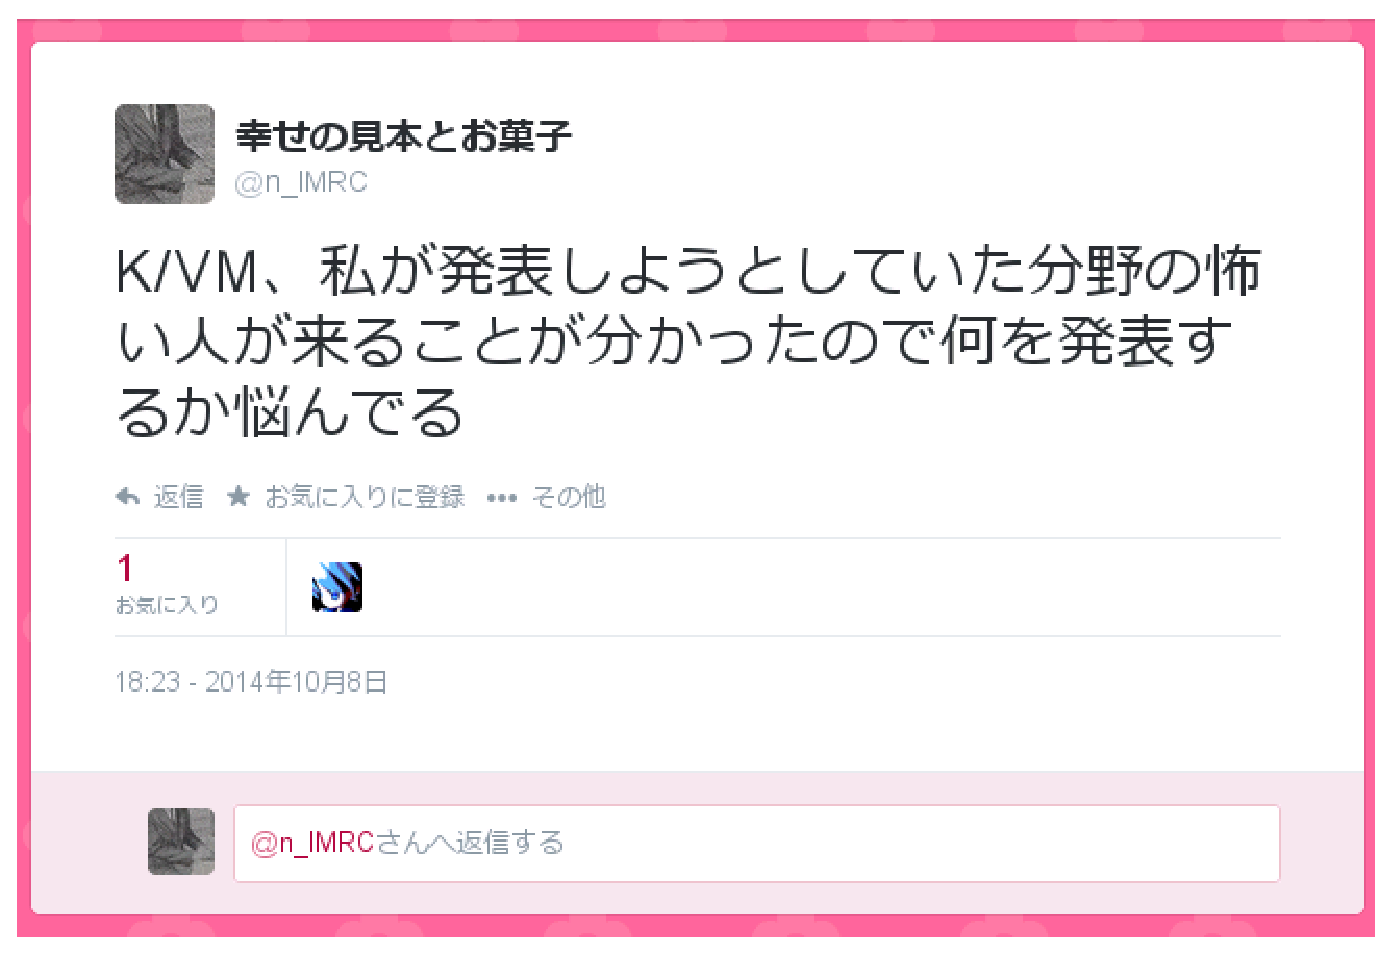
\includegraphics[width=\textwidth]{1.eps}
\end{figure}
\end{frame}
\begin{frame}\frametitle{今日話す内容}
\begin{itemize}
\item USBキーボード to Bluetooth コンバータの製作...?
\begin{itemize}
\item 45分持たない
\item ボツ
\end{itemize}
\end{itemize}
\end{frame}
\begin{frame}\frametitle{今日話す内容}
\begin{figure}[htb]
\centering
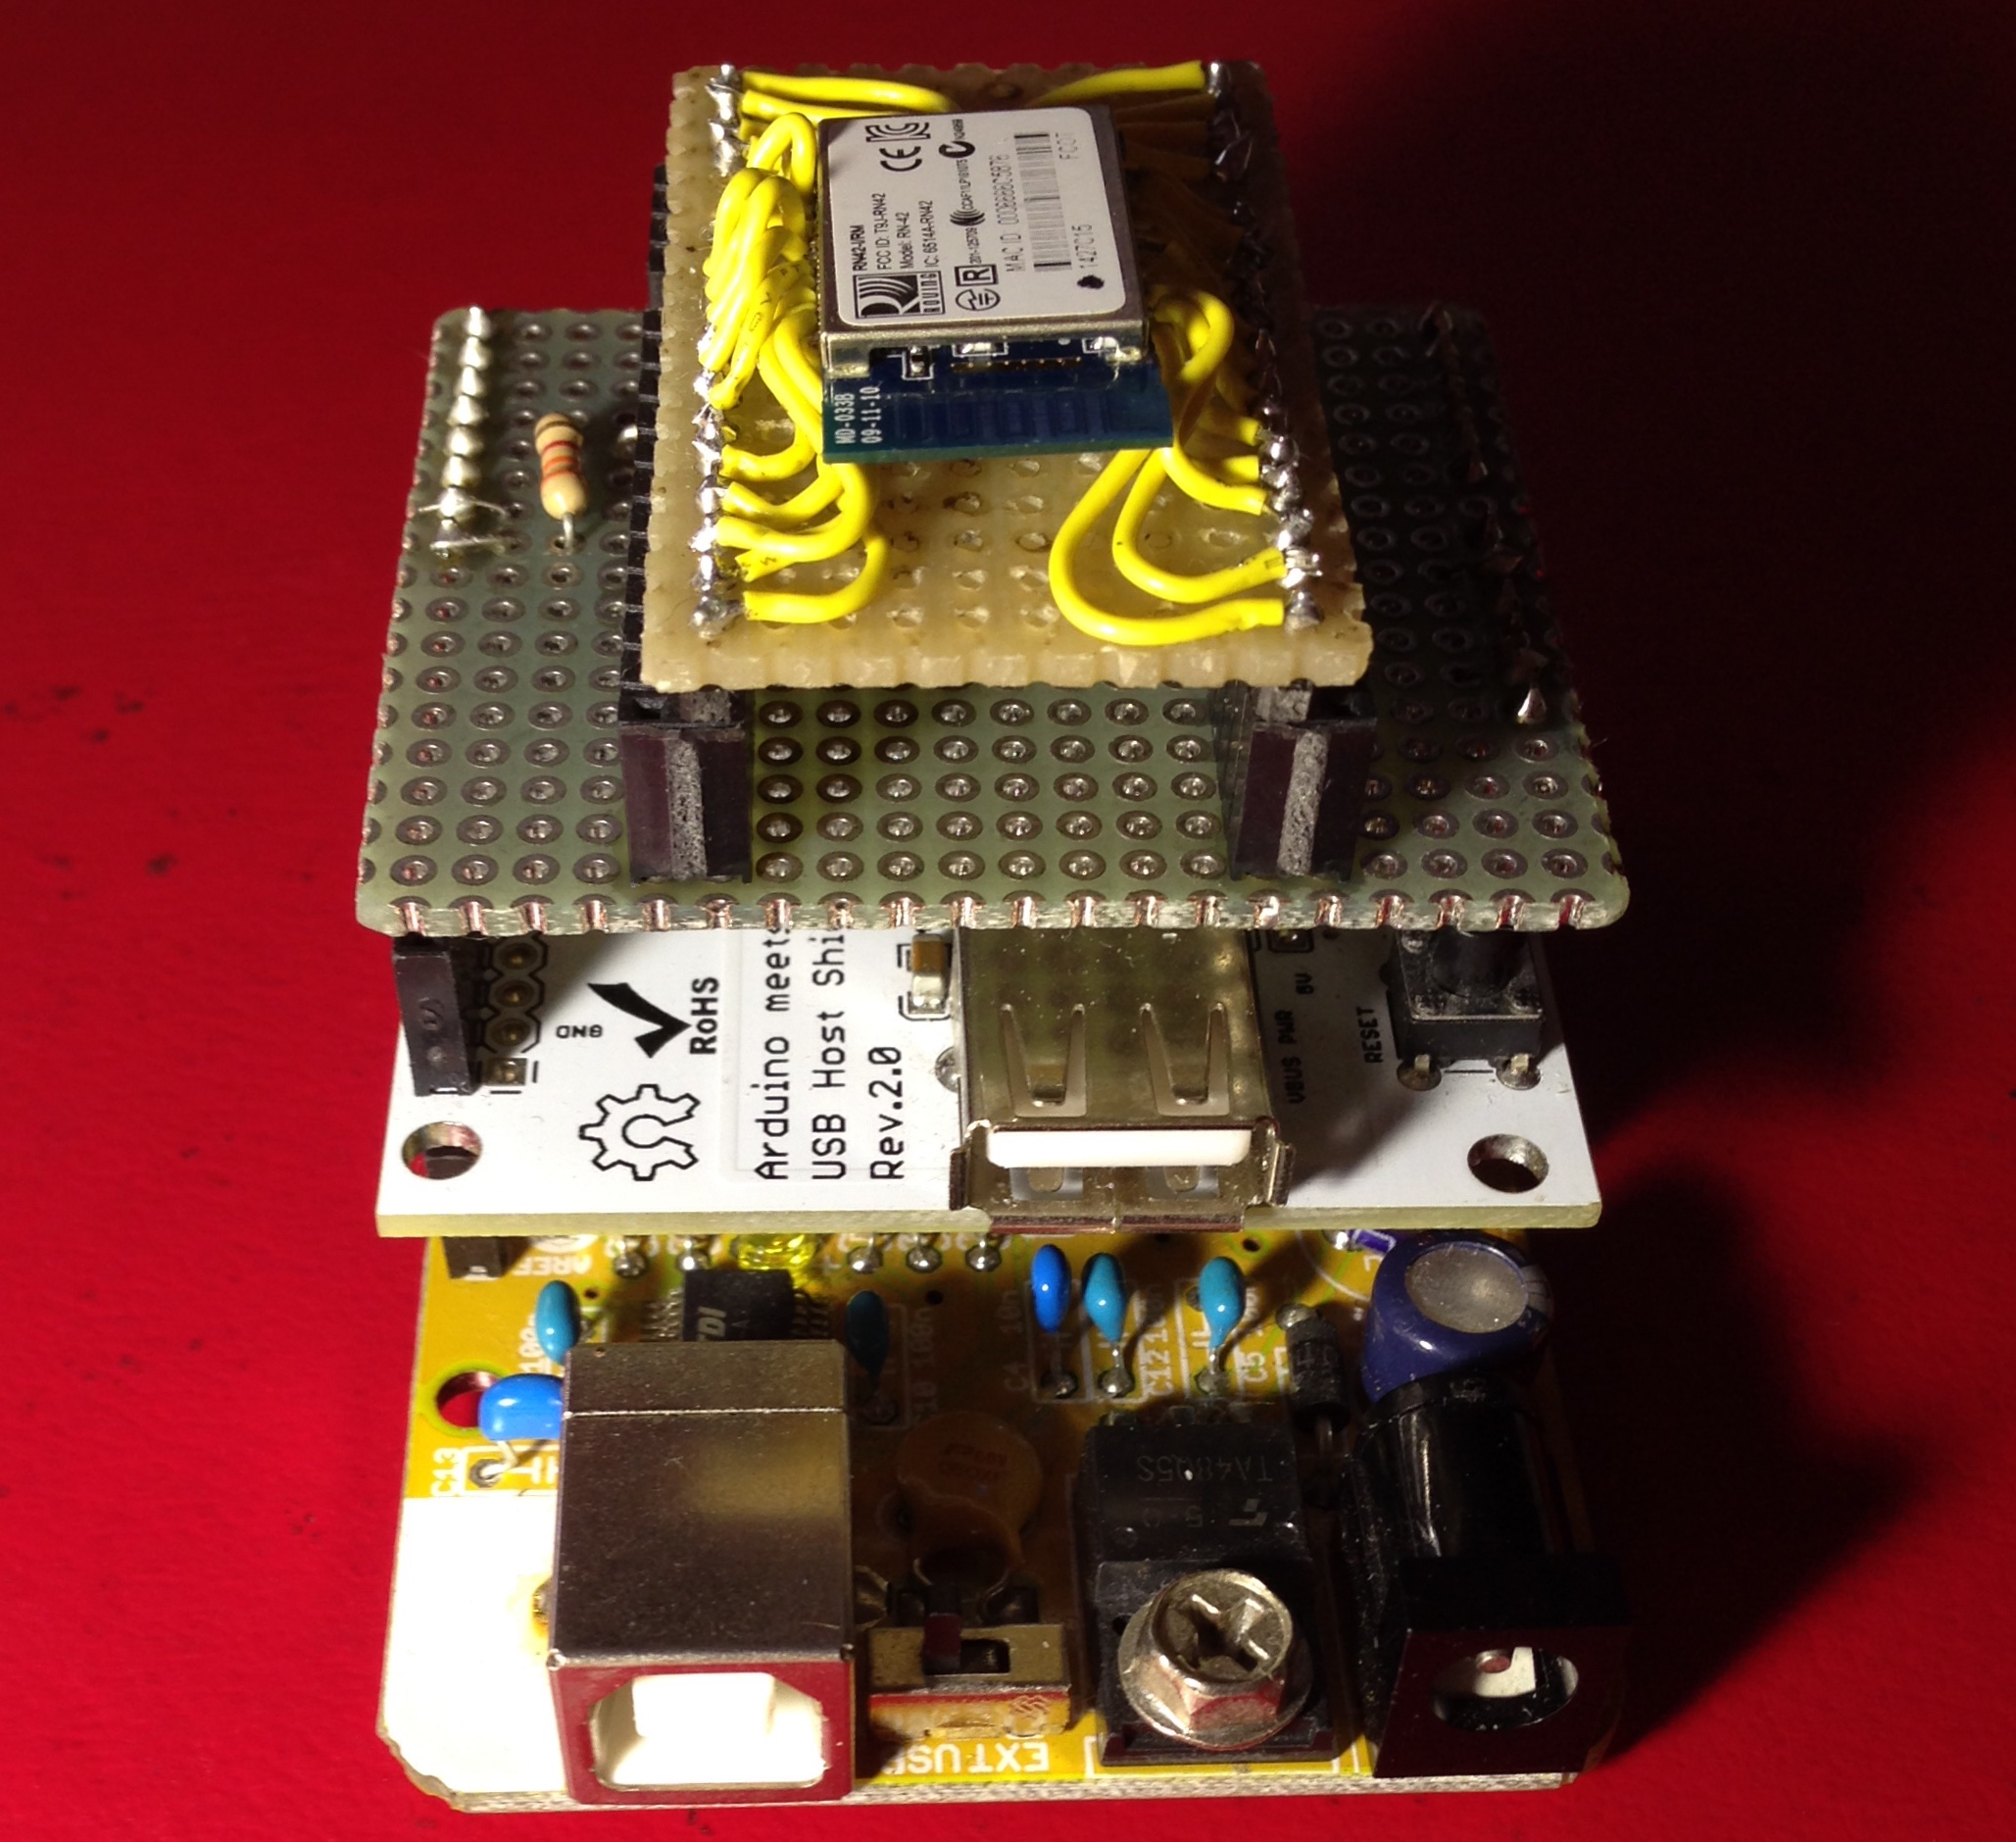
\includegraphics[width=0.7\textwidth]{bt.eps}
\end{figure}
\end{frame}

\begin{frame}\frametitle{今日話す内容}
\begin{itemize}
	\item initスクリプトを書いてRaspberryPiのOSをUSB HDDから起動できるようにした話...?
	\begin{itemize}
		\item 新規性がない
		\item 45分持たない
		\item ボツ
	\end{itemize}
\end{itemize}
\end{frame}
\begin{frame}\frametitle{今日話す内容}
\begin{itemize}
	\item framebufferをpngやjpegに変換するプログラムを書き、mjpg\_streamer経由でストリーミングできるようにした話...?
	\begin{itemize}
		\item 最近のTLの風潮はsixel
		\item 45分持たない
		\item ボツ
	\end{itemize}
\end{itemize}
\end{frame}

\begin{frame}\frametitle{今日話す内容}
\begin{itemize}
\item 45分の内に複数テーマを話す...?
\begin{itemize}
\item 45分話したかった方に申し訳ない
\begin{itemize}
\item マサカリは怖いけど...
\end{itemize}
\end{itemize}
\end{itemize}
\end{frame}
\begin{frame}\frametitle{今日話す内容}
\begin{figure}[htb]
\centering
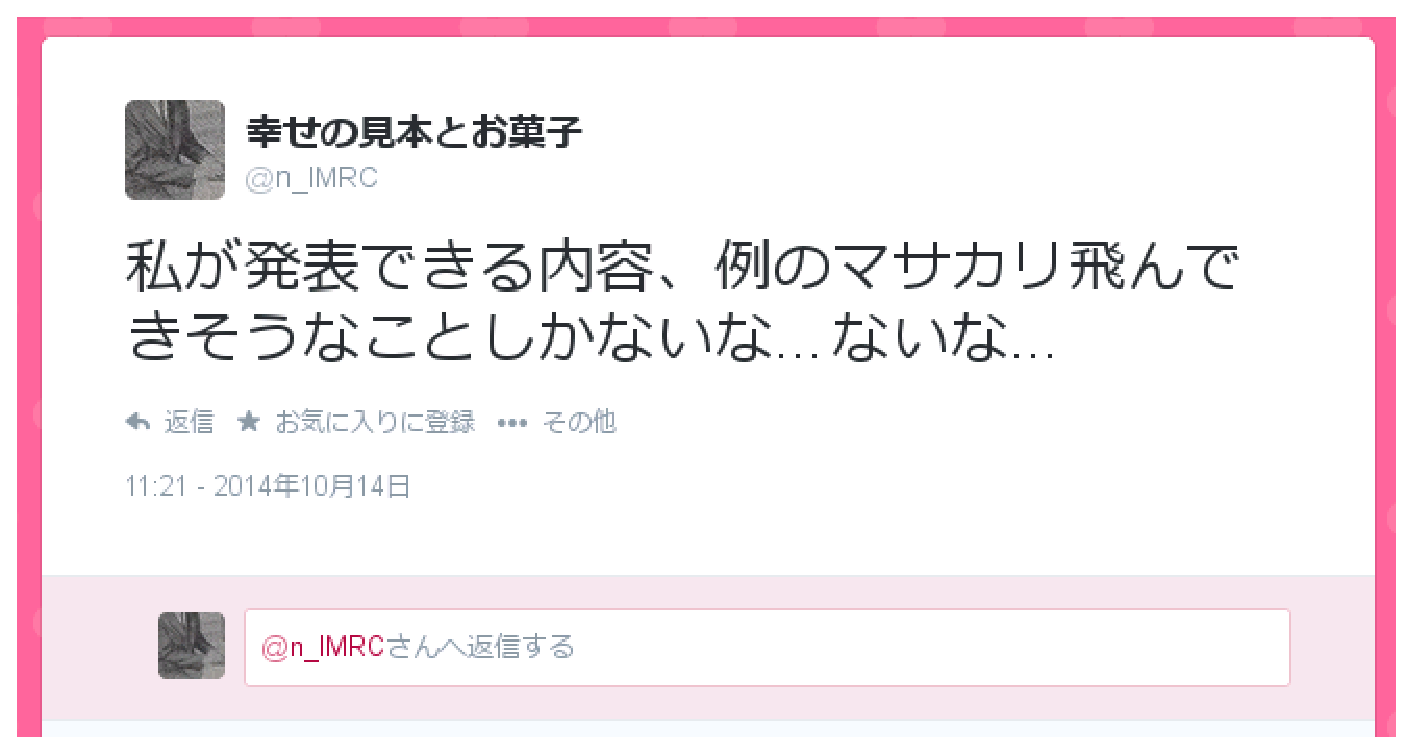
\includegraphics[width=\textwidth]{2.eps}
\end{figure}
\end{frame}
\begin{frame}\frametitle{今日話す内容}
\centering
\large
\vspace*{\fill}
XeonPhiの性能が出にくい話
\vspace*{\fill}
\end{frame}

\begin{frame}\frametitle{並列計算とは}
\begin{itemize}
\item 複数のCPUやスレッドで分散して処理
\item 実行時間の短縮が目的
\begin{itemize}
\item 理想は \textbf{(元の実行時間)/n}
\item 通信やアルゴリズムのオーバーヘッドにより、現実的に不可能
\end{itemize}
\end{itemize}
\end{frame}

\begin{frame}\frametitle{並列計算のための環境}
\begin{itemize}
\item 数値計算においてはMPI, OpenMP, pthread等の高レベルなライブラリ
\item 筑波大学がdirectiveベースの、MPIによる並列言語XcalableMPを開発中
\item CPU間通信にNUMAを使うことも
\end{itemize}
\end{frame}

\begin{frame}\frametitle{スーパーコンピュータ}
\begin{itemize}
\item (多少高性能な)コンピュータの集まり
\begin{itemize}
\item もちろん並列計算
\end{itemize}
\item 現在、筑波大学はHA-PACSとCOMAを運用している
\begin{itemize}
\item 昨年度までT2K-Tsukubaが運用されていた
\end{itemize}
\end{itemize}
\end{frame}

\begin{frame}\frametitle{T2K-Tsukuba}
\small
1ノード: quad-core AMD Opteron $\times$ 4
\begin{figure}[htb]
\centering
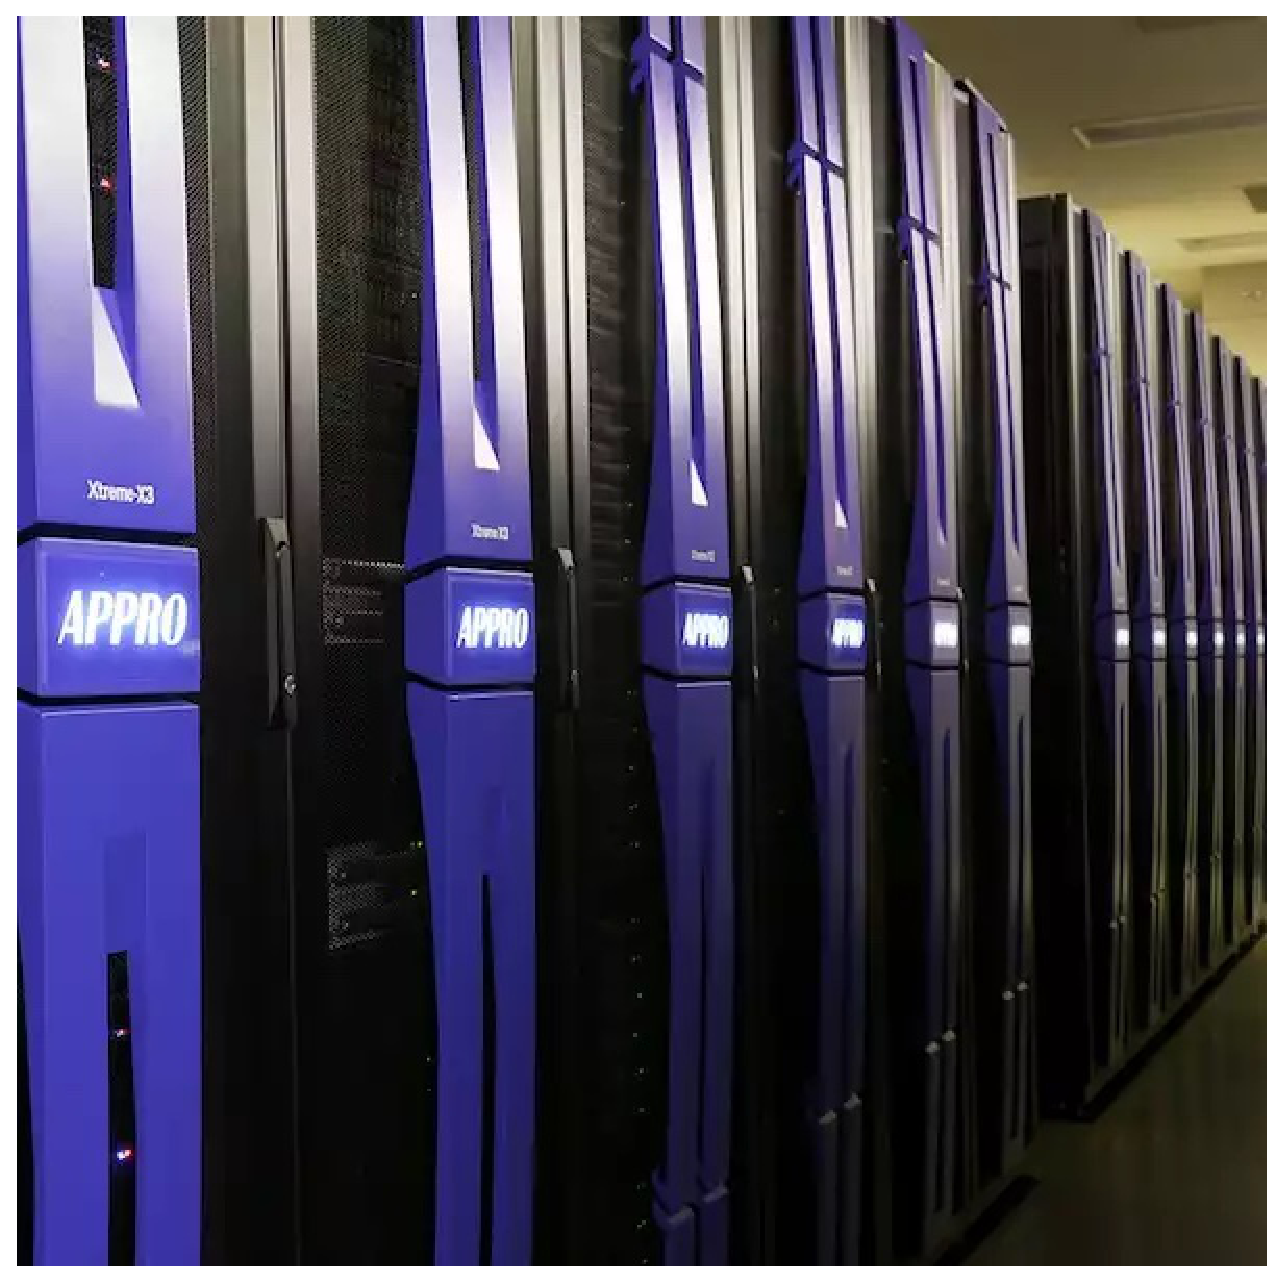
\includegraphics[height=0.6\textheight]{t2kt.eps}
\end{figure}
\end{frame}

\begin{frame}\frametitle{HA-PACS}
\small
1ノード: NVIDIA M2090(Fermi) $\times$ 4
\begin{figure}[htb]
\centering
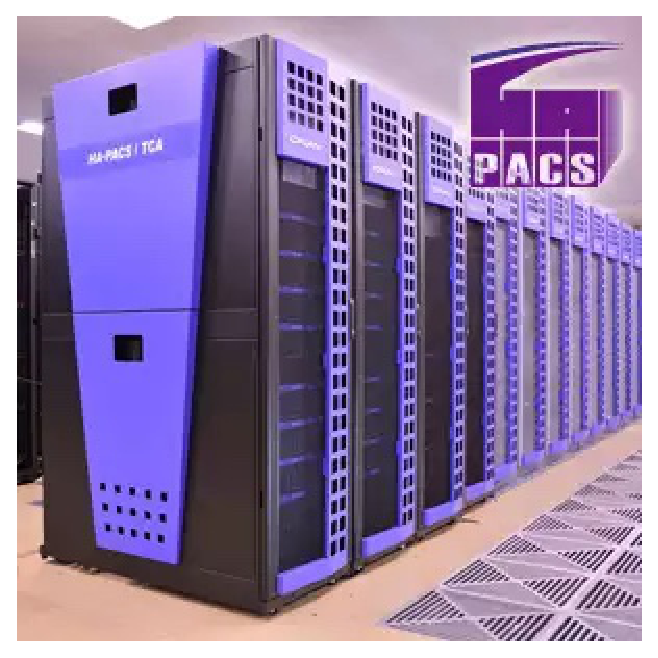
\includegraphics[height=0.6\textheight]{hapacs.eps}
\end{figure}
\end{frame}

\begin{frame}\frametitle{COMA}
\small
1ノード: Intel Xeon Phi $\times$ 2
\begin{figure}[htb]
\centering
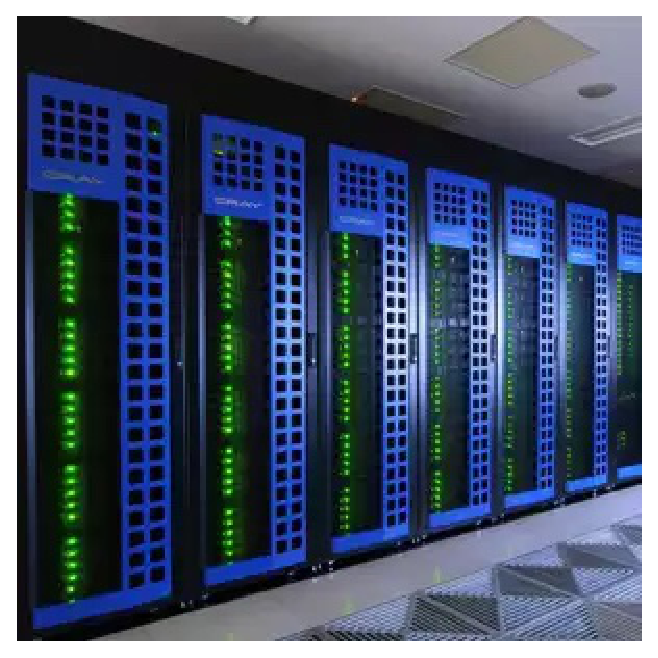
\includegraphics[height=0.6\textheight]{coma.eps}
\end{figure}
\end{frame}

%\setcounter{framenumber}{\value{finalframe}}
\end{document}
